Die Versuchsdurchführung erfolgt im Gebäude C12, Raum 3.28. Das verwendete Gerät ist der Phenom XL G2.\\
Das Experiment wird in zwei Abschnitten durchgeführt:\\
\begin{enumerate}
\item Untersuchung die Strukturen folgender Teile des SiC-Mosfet (\hyperref[Abb.3: Positionierung der Messpositionen auf SiC-Mosfet]{Abbildung 3}):
    \subitem 1.1. Gate Pad
    \subitem 1.2. Sinterpad
    \subitem 1.3. Source Pad
\item Analyse einer gesinterten Sinterpaste in einem Al-Tiegel mithilfe von EDX Analyse(\hyperref[Abb.4: Probe aus Sinterpaste in Aluminiumtiegel]{Abbildung 4}):
\end{enumerate}
\vspace{0.5cm}
\begin{figure}[H]
    \centering
    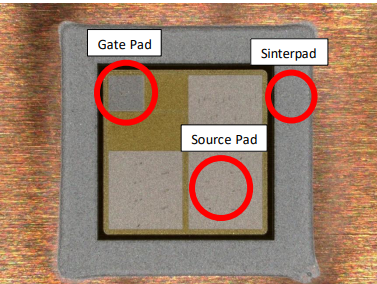
\includegraphics[scale=0.95]{Bilder/Screenshot 2025-04-10 185117}
    \caption{Positionierung der Messpositionen auf SiC-Mosfet\cite{key}}
    \vspace{0.2cm}
    \label{Abb.3: Positionierung der Messpositionen auf SiC-Mosfet}
\end{figure} 
\begin{figure}[H]
    \centering
    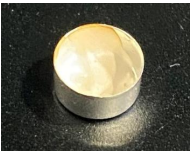
\includegraphics[scale=0.95]{Bilder/Screenshot 2025-04-10 190248}
    \caption{Probe aus Sinterpaste in Aluminiumtiegel\cite{key}}
    
    \vspace{0.2cm}
    \label{Abb.4: Probe aus Sinterpaste in Aluminiumtiegel}
\end{figure} 
\subsection{Struktur Untersuchung}
Die Untersuchung begann mit dem ersten Teil des MOSFETs, dem Gate-Pad. Dabei wurde – wie bei jedem anderen Teil – das gleiche Verfahren angewendet: 
Zunächst erfolgte die Aufnahme mit dem BSE-Detektor (Backscattered Electrons) bei drei verschiedenen Vergrößerungsstufen:
\begin{enumerate}
    \item 4000x
    \item 10000x
    \item 15000x 
\end{enumerate}
Anschließend wurde die Aufnahme mit dem SE-Detektor (Sekundärelektronen) unter den gleichen Vergrößerungsstufen durchgeführt. 
Daraufhin erfolgte eine Analyse mittels EDX (energie-dispersive Röntgenspektroskopie), um die chemische Zusammensetzung der jeweiligen Strukturen zu bestimmen.\\
Zu guter Letzt wurde die gesinterte Sinterpaste in einem Aluminium-Tiegel mittels EDX analysiert, wobei ihre chemische Zusammensetzung vollständig bestimmt wurde.
